% Created by tikzDevice version 0.12 on 2019-03-27 17:35:13
% !TEX encoding = UTF-8 Unicode
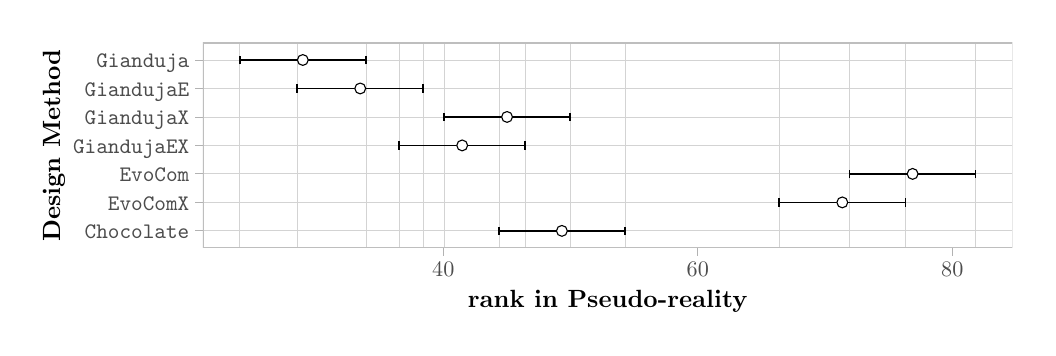
\begin{tikzpicture}[x=1pt,y=1pt]
\definecolor{fillColor}{RGB}{255,255,255}
\path[use as bounding box,fill=fillColor,fill opacity=0.00] (0,0) rectangle (361.35,108.41);
\begin{scope}
\path[clip] (  0.00,  0.00) rectangle (361.35,108.40);
\definecolor{drawColor}{RGB}{255,255,255}
\definecolor{fillColor}{RGB}{255,255,255}

\path[draw=drawColor,line width= 0.6pt,line join=round,line cap=round,fill=fillColor] (  0.00,  0.00) rectangle (361.35,108.40);
\end{scope}
\begin{scope}
\path[clip] ( 63.34, 28.81) rectangle (355.85,102.90);
\definecolor{fillColor}{RGB}{255,255,255}

\path[fill=fillColor] ( 63.34, 28.81) rectangle (355.85,102.90);
\definecolor{drawColor}{RGB}{211,211,211}

\path[draw=drawColor,line width= 0.3pt,line join=round] ( 63.34, 55.57) --
	(355.85, 55.57);

\path[draw=drawColor,line width= 0.3pt,line join=round] ( 63.34, 45.27) --
	(355.85, 45.27);

\path[draw=drawColor,line width= 0.3pt,line join=round] ( 63.34, 96.73) --
	(355.85, 96.73);

\path[draw=drawColor,line width= 0.3pt,line join=round] ( 63.34, 86.44) --
	(355.85, 86.44);

\path[draw=drawColor,line width= 0.3pt,line join=round] ( 63.34, 76.15) --
	(355.85, 76.15);

\path[draw=drawColor,line width= 0.3pt,line join=round] ( 63.34, 65.86) --
	(355.85, 65.86);

\path[draw=drawColor,line width= 0.3pt,line join=round] ( 63.34, 34.98) --
	(355.85, 34.98);

\path[draw=drawColor,line width= 0.2pt,line join=round] (215.82, 28.81) -- (215.82,102.90);

\path[draw=drawColor,line width= 0.2pt,line join=round] (342.55, 28.81) -- (342.55,102.90);

\path[draw=drawColor,line width= 0.2pt,line join=round] (317.15, 28.81) -- (317.15,102.90);

\path[draw=drawColor,line width= 0.2pt,line join=round] (122.21, 28.81) -- (122.21,102.90);

\path[draw=drawColor,line width= 0.2pt,line join=round] (142.95, 28.81) -- (142.95,102.90);

\path[draw=drawColor,line width= 0.2pt,line join=round] (179.80, 28.81) -- (179.80,102.90);

\path[draw=drawColor,line width= 0.2pt,line join=round] (196.00, 28.81) -- (196.00,102.90);

\path[draw=drawColor,line width= 0.2pt,line join=round] (170.25, 28.81) -- (170.25,102.90);

\path[draw=drawColor,line width= 0.2pt,line join=round] (296.99, 28.81) -- (296.99,102.90);

\path[draw=drawColor,line width= 0.2pt,line join=round] (271.59, 28.81) -- (271.59,102.90);

\path[draw=drawColor,line width= 0.2pt,line join=round] ( 76.64, 28.81) -- ( 76.64,102.90);

\path[draw=drawColor,line width= 0.2pt,line join=round] ( 97.39, 28.81) -- ( 97.39,102.90);

\path[draw=drawColor,line width= 0.2pt,line join=round] (134.23, 28.81) -- (134.23,102.90);

\path[draw=drawColor,line width= 0.2pt,line join=round] (150.44, 28.81) -- (150.44,102.90);
\definecolor{drawColor}{RGB}{0,0,0}

\path[draw=drawColor,line width= 0.6pt,line join=round] (215.82, 33.44) --
	(215.82, 36.53);

\path[draw=drawColor,line width= 0.6pt,line join=round] (215.82, 34.98) --
	(170.25, 34.98);

\path[draw=drawColor,line width= 0.6pt,line join=round] (170.25, 33.44) --
	(170.25, 36.53);

\path[draw=drawColor,line width= 0.6pt,line join=round] (342.55, 54.02) --
	(342.55, 57.11);

\path[draw=drawColor,line width= 0.6pt,line join=round] (342.55, 55.57) --
	(296.99, 55.57);

\path[draw=drawColor,line width= 0.6pt,line join=round] (296.99, 54.02) --
	(296.99, 57.11);

\path[draw=drawColor,line width= 0.6pt,line join=round] (317.15, 43.73) --
	(317.15, 46.82);

\path[draw=drawColor,line width= 0.6pt,line join=round] (317.15, 45.27) --
	(271.59, 45.27);

\path[draw=drawColor,line width= 0.6pt,line join=round] (271.59, 43.73) --
	(271.59, 46.82);

\path[draw=drawColor,line width= 0.6pt,line join=round] (122.21, 95.19) --
	(122.21, 98.27);

\path[draw=drawColor,line width= 0.6pt,line join=round] (122.21, 96.73) --
	( 76.64, 96.73);

\path[draw=drawColor,line width= 0.6pt,line join=round] ( 76.64, 95.19) --
	( 76.64, 98.27);

\path[draw=drawColor,line width= 0.6pt,line join=round] (142.95, 84.90) --
	(142.95, 87.98);

\path[draw=drawColor,line width= 0.6pt,line join=round] (142.95, 86.44) --
	( 97.39, 86.44);

\path[draw=drawColor,line width= 0.6pt,line join=round] ( 97.39, 84.90) --
	( 97.39, 87.98);

\path[draw=drawColor,line width= 0.6pt,line join=round] (179.80, 64.31) --
	(179.80, 67.40);

\path[draw=drawColor,line width= 0.6pt,line join=round] (179.80, 65.86) --
	(134.23, 65.86);

\path[draw=drawColor,line width= 0.6pt,line join=round] (134.23, 64.31) --
	(134.23, 67.40);

\path[draw=drawColor,line width= 0.6pt,line join=round] (196.00, 74.60) --
	(196.00, 77.69);

\path[draw=drawColor,line width= 0.6pt,line join=round] (196.00, 76.15) --
	(150.44, 76.15);

\path[draw=drawColor,line width= 0.6pt,line join=round] (150.44, 74.60) --
	(150.44, 77.69);

\path[draw=drawColor,line width= 0.4pt,line join=round,line cap=round,fill=fillColor] (193.04, 34.98) circle (  1.96);

\path[draw=drawColor,line width= 0.4pt,line join=round,line cap=round,fill=fillColor] (319.77, 55.57) circle (  1.96);

\path[draw=drawColor,line width= 0.4pt,line join=round,line cap=round,fill=fillColor] (294.37, 45.27) circle (  1.96);

\path[draw=drawColor,line width= 0.4pt,line join=round,line cap=round,fill=fillColor] ( 99.42, 96.73) circle (  1.96);

\path[draw=drawColor,line width= 0.4pt,line join=round,line cap=round,fill=fillColor] (120.17, 86.44) circle (  1.96);

\path[draw=drawColor,line width= 0.4pt,line join=round,line cap=round,fill=fillColor] (157.01, 65.86) circle (  1.96);

\path[draw=drawColor,line width= 0.4pt,line join=round,line cap=round,fill=fillColor] (173.22, 76.15) circle (  1.96);
\definecolor{drawColor}{RGB}{190,190,190}

\path[draw=drawColor,line width= 0.6pt,line join=round,line cap=round] ( 63.34, 28.81) rectangle (355.85,102.90);
\end{scope}
\begin{scope}
\path[clip] (  0.00,  0.00) rectangle (361.35,108.41);
\definecolor{drawColor}{gray}{0.30}

\node[text=drawColor,anchor=base east,inner sep=0pt, outer sep=0pt, scale=  0.80] at ( 58.39, 52.81) {\texttt{EvoCom}};

\node[text=drawColor,anchor=base east,inner sep=0pt, outer sep=0pt, scale=  0.80] at ( 58.39, 42.52) {\texttt{EvoComX}};

\node[text=drawColor,anchor=base east,inner sep=0pt, outer sep=0pt, scale=  0.80] at ( 58.39, 93.98) {\texttt{Gianduja}};

\node[text=drawColor,anchor=base east,inner sep=0pt, outer sep=0pt, scale=  0.80] at ( 58.39, 83.68) {\texttt{GiandujaE}};

\node[text=drawColor,anchor=base east,inner sep=0pt, outer sep=0pt, scale=  0.80] at ( 58.39, 73.39) {\texttt{GiandujaX}};

\node[text=drawColor,anchor=base east,inner sep=0pt, outer sep=0pt, scale=  0.80] at ( 58.39, 63.10) {\texttt{GiandujaEX}};

\node[text=drawColor,anchor=base east,inner sep=0pt, outer sep=0pt, scale=  0.80] at ( 58.39, 32.23) {\texttt{Chocolate}};
\end{scope}
\begin{scope}
\path[clip] (  0.00,  0.00) rectangle (361.35,108.41);
\definecolor{drawColor}{gray}{0.70}

\path[draw=drawColor,line width= 0.3pt,line join=round] ( 60.59, 55.57) --
	( 63.34, 55.57);

\path[draw=drawColor,line width= 0.3pt,line join=round] ( 60.59, 45.27) --
	( 63.34, 45.27);

\path[draw=drawColor,line width= 0.3pt,line join=round] ( 60.59, 96.73) --
	( 63.34, 96.73);

\path[draw=drawColor,line width= 0.3pt,line join=round] ( 60.59, 86.44) --
	( 63.34, 86.44);

\path[draw=drawColor,line width= 0.3pt,line join=round] ( 60.59, 76.15) --
	( 63.34, 76.15);

\path[draw=drawColor,line width= 0.3pt,line join=round] ( 60.59, 65.86) --
	( 63.34, 65.86);

\path[draw=drawColor,line width= 0.3pt,line join=round] ( 60.59, 34.98) --
	( 63.34, 34.98);
\end{scope}
\begin{scope}
\path[clip] (  0.00,  0.00) rectangle (361.35,108.41);
\definecolor{drawColor}{gray}{0.70}

\path[draw=drawColor,line width= 0.3pt,line join=round] (150.17, 26.06) --
	(150.17, 28.81);

\path[draw=drawColor,line width= 0.3pt,line join=round] (242.14, 26.06) --
	(242.14, 28.81);

\path[draw=drawColor,line width= 0.3pt,line join=round] (334.11, 26.06) --
	(334.11, 28.81);
\end{scope}
\begin{scope}
\path[clip] (  0.00,  0.00) rectangle (361.35,108.41);
\definecolor{drawColor}{gray}{0.30}

\node[text=drawColor,anchor=base,inner sep=0pt, outer sep=0pt, scale=  0.80] at (150.17, 18.35) {40};

\node[text=drawColor,anchor=base,inner sep=0pt, outer sep=0pt, scale=  0.80] at (242.14, 18.35) {60};

\node[text=drawColor,anchor=base,inner sep=0pt, outer sep=0pt, scale=  0.80] at (334.11, 18.35) {80};
\end{scope}
\begin{scope}
\path[clip] (  0.00,  0.00) rectangle (361.35,108.41);
\definecolor{drawColor}{RGB}{0,0,0}

\node[text=drawColor,anchor=base,inner sep=0pt, outer sep=0pt, scale=  0.90] at (209.60,  7.44) {\bfseries rank in Pseudo-reality};
\end{scope}
\begin{scope}
\path[clip] (  0.00,  0.00) rectangle (361.35,108.41);
\definecolor{drawColor}{RGB}{0,0,0}

\node[text=drawColor,rotate= 90.00,anchor=base,inner sep=0pt, outer sep=0pt, scale=  0.90] at ( 11.71, 65.86) {\bfseries Design Method};
\end{scope}
\end{tikzpicture}
